\documentclass[a4paper, 12pt]{article}
% packages
\usepackage{amssymb}
\usepackage[fleqn]{mathtools}
\usepackage{tikz}
\usepackage{enumerate}
\usepackage{bussproofs}
\usepackage{xcolor}
\usepackage[margin=1.3cm]{geometry}
\usepackage{logicproof}
\usepackage{diagbox}
\usepackage{listings}
\usepackage{graphicx}
\usepackage{lstautogobble}
\usepackage{hyperref}
\usepackage{multirow}
\usepackage{tipa}
\usetikzlibrary{decorations.pathreplacing, arrows, shapes.gates.logic.US, circuits.logic.US, calc, automata, positioning, intersections}

% shorthand for verbatim
% this clashes with logicproof, so maybe fix this at some point?
\catcode`~=\active
\def~#1~{\texttt{#1}}

% code listing
\lstdefinestyle{main}{
    numberstyle=\tiny,
    breaklines=true,
    showspaces=false,
    showstringspaces=false,
    tabsize=2,
    numbers=left,
    basicstyle=\ttfamily,
    columns=fixed,
    fontadjust=true,
    basewidth=0.5em,
    autogobble,
    xleftmargin=3.0ex,
    mathescape=true
}
\newcommand{\dollar}{\mbox{\textdollar}} %
\lstset{style=main}

% augmented matrix
\makeatletter
\renewcommand*\env@matrix[1][*\c@MaxMatrixCols c]{%
\hskip -\arraycolsep
\let\@ifnextchar\new@ifnextchar
\array{#1}}
\makeatother

% ceiling / floor
\DeclarePairedDelimiter{\ceil}{\lceil}{\rceil}
\DeclarePairedDelimiter{\floor}{\lfloor}{\rfloor}

% custom commands
\newcommand{\indefint}[2]{\int #1 \, \mathrm{d}#2}
\newcommand{\defint}[4]{\int_{#1}^{#2} #3 \, \mathrm{d}#4}
\newcommand{\pdif}[2]{\frac{\partial #1}{\partial #2}}
\newcommand{\dif}[2]{\frac{\mathrm{d}#1}{\mathrm{d}#2}}
\newcommand{\limit}[2]{\raisebox{0.5ex}{\scalebox{0.8}{$\displaystyle{\lim_{#1 \to #2}}$}}}
\newcommand{\summation}[2]{\sum\limits_{#1}^{#2}}
\newcommand{\product}[2]{\prod\limits_{#1}^{#2}}
\newcommand{\intbracket}[3]{\left[#3\right]_{#1}^{#2}}
\newcommand{\ulsmash}[1]{\underline{\smash{#1}}}

\newcommand{\powerset}[0]{\wp}
\renewcommand{\emptyset}[0]{\varnothing}

\makeatletter
\newsavebox{\@brx}
\newcommand{\llangle}[1][]{\savebox{\@brx}{\(\m@th{#1\langle}\)}%
  \mathopen{\copy\@brx\kern-0.5\wd\@brx\usebox{\@brx}}}
\newcommand{\rrangle}[1][]{\savebox{\@brx}{\(\m@th{#1\rangle}\)}%
  \mathclose{\copy\@brx\kern-0.5\wd\@brx\usebox{\@brx}}}
\makeatother
\newcommand{\lla}{\llangle}
\newcommand{\rra}{\rrangle}
\newcommand{\la}{\langle}
\newcommand{\ra}{\rangle}
\newcommand{\crnr}[1]{\text{\textopencorner} #1 \text{\textcorner}}
\newcommand{\laplace}{\mathcal{L}}
\newcommand{\fourier}{\mathcal{F}}

\newcommand{\mat}[1]{\boldsymbol{#1}}
\renewcommand{\vec}[1]{\boldsymbol{#1}}
\newcommand{\rowt}[1]{\begin{bmatrix}
    #1
\end{bmatrix}^\top}

\newcommand{\unaryproof}[2]{\AxiomC{#1} \UnaryInfC{#2} \DisplayProof}
\newcommand{\binaryproof}[3]{\AxiomC{#1} \AxiomC{#2} \BinaryInfC{#3} \DisplayProof}
\newcommand{\trinaryproof}[4]{\AxiomC{#1} \AxiomC{#2} \AxiomC{#3} \TrinaryInfC{#4} \DisplayProof}

\newcommand{\axiom}[1]{\AxiomC{#1}}
\newcommand{\unary}[1]{\UnaryInfC{#1}}
\newcommand{\binary}[1]{\BinaryInfC{#1}}
\newcommand{\trinary}[1]{\TrinaryInfC{#1}}
\newcommand{\quaternary}[1]{\QuaternaryInfC{#1}}
\newcommand{\quinary}[1]{\QuinaryInfC{#1}}
\newcommand{\dproof}[0]{\DisplayProof}

\newcommand{\bnfsep}[0]{\ |\ }
\newcommand{\lrbt}[0]{\ \bullet\ }
\newcommand{\concsep}[0]{\ ||\ }
\newcommand{\ttbs}{\char`\\}

\newcommand{\violet}[1]{\textcolor{violet}{#1}}
\newcommand{\blue}[1]{\textcolor{blue}{#1}}
\newcommand{\red}[1]{\textcolor{red}{#1}}

% no indent
\setlength\parindent{0pt}

% reasoning proofs
\usepackage{ltablex}
\usepackage{environ}
\keepXColumns
\NewEnviron{reasoning}{
    \begin{tabularx}{\textwidth}{rlX}
        \BODY
    \end{tabularx}
}
\newcommand{\proofline}[3]{$(#1)$ & $#2$ & \hfill #3 \medskip \\}
\newcommand{\proofarbitrary}[1]{& take arbitrary $#1$ \medskip \\}
\newcommand{\prooftext}[1]{\multicolumn{3}{l}{#1} \medskip \\}
\newcommand{\proofmath}[3]{$#1$ & = $#2$ & \hfill #3 \medskip \\}
\newcommand{\prooftherefore}[1]{& $\therefore #1$ \medskip \\}
\newcommand{\proofbc}[0]{\prooftext{\textbf{Base Case}}}
\newcommand{\proofis}[0]{\prooftext{\textbf{Inductive Step}}}

% reasoning er diagrams
\newcommand{\nattribute}[4]{
    \node[draw, state, inner sep=0cm, minimum size=0.2cm, label=#3:{#4}] (#1) at (#2) {};
}
\newcommand{\mattribute}[4]{
    \node[draw, state, accepting, inner sep=0cm, minimum size=0.2cm, label=#3:{#4}] (#1) at (#2) {};
}
\newcommand{\dattribute}[4]{
    \node[draw, state, dashed, inner sep=0cm, minimum size=0.2cm, label=#3:{#4}] (#1) at (#2) {};
}
\newcommand{\entity}[3]{
    \node[] (#1-c) at (#2) {#3};
    \node[inner sep=0cm] (#1-l) at ($(#1-c) + (-1, 0)$) {};
    \node[inner sep=0cm] (#1-r) at ($(#1-c) + (1, 0)$) {};
    \node[inner sep=0cm] (#1-u) at ($(#1-c) + (0, 0.5)$) {};
    \node[inner sep=0cm] (#1-d) at ($(#1-c) + (0, -0.5)$) {};
    \draw
    ($(#1-c) + (-1, 0.5)$) -- ($(#1-c) + (1, 0.5)$) -- ($(#1-c) + (1, -0.5)$) -- ($(#1-c) + (-1, -0.5)$) -- cycle;
}
\newcommand{\relationship}[3]{
    \node[] (#1-c) at (#2) {#3};
    \node[inner sep=0cm] (#1-l) at ($(#1-c) + (-1, 0)$) {};
    \node[inner sep=0cm] (#1-r) at ($(#1-c) + (1, 0)$) {};
    \node[inner sep=0cm] (#1-u) at ($(#1-c) + (0, 1)$) {};
    \node[inner sep=0cm] (#1-d) at ($(#1-c) + (0, -1)$) {};
    \draw
    ($(#1-c) + (-1, 0)$) -- ($(#1-c) + (0, 1)$) -- ($(#1-c) + (1, 0)$) -- ($(#1-c) + (0, -1)$) -- cycle;
}

% actual document
\begin{document}
    \section*{CO211 - Operating Systems}
        \subsection*{4th October 2019}
            \subsubsection*{Outline of the Course}
                \begin{itemize}
                    \itemsep0em
                    \item overview and introduction \hfill structure, case studies
                    \item processes and threads \hfill abstractions that an OS uses to execute code
                    \item inter-process communication (IPC) \hfill allows multiple processes to communicate with each other
                    \item memory management \hfill allocation, abstraction for virtual memory, paging
                    \item device management \hfill types, drivers
                    \item disk management \hfill scheduling, caching, RAID
                    \item file systems \hfill basic abstractions for storage and implementation
                    \item security \hfill authentication, access control
                \end{itemize}
                Note that this follows a similar structure to most OS courses, and therefore we can reference content from other sources.
                \textit{Operating Systems: Three Easy Pieces} is recommended, as it bridges between this course and the PintOS lab.
            \subsubsection*{Overview}
                The general overview is that there is a system bus that interconnects different hardware components (including CPU and memory), and allows for communication between them.
                \medskip

                The operating system provides abstractions for programs to use, meaning that they do not have to deal with the complex hardware.
                For example, a process abstraction expects an interface to the hardware, which allows programs to be used on different hardware.
                This means that the OS will need how to to control the hardware with drivers.
                The operating system has the following goals;
                \begin{enumerate}[(1)]
                    \itemsep0em
                    \item \textbf{managing resources}
                        \medskip

                        The operating system must be able to expose the resources efficiently to the application, and also share these resources fairly.
                        Some examples are;
                        \begin{itemize}
                            \itemsep0em
                            \item CPU (multiple cores) \hfill should decide what runs on each hardware thread
                            \item memory \hfill cache, RAM
                            \item I/O devices \hfill displays (GPUs), network interfaces
                            \item internal devices \hfill clocks, timers, interrupt controllers
                            \item persistent storage
                        \end{itemize}
                        OS uses both time and space multiplexing for sharing.
                        An example for the former is how the effect of parallelism can be achieved with a single CPU core by splitting up the time allocated per process, and an example for the latter is splitting up memory for each process.
                        \medskip

                        On the other hand, with allocation, the OS must also support simultaneous resource access (such as to disks, RAM, network etc.).
                        Continuing from this, it must also offer mutual exclusion, thus protecting risky operations (such as file writing).
                        Generally, the OS aims to protect against corruption.
                        \medskip

                        Finally, the operating system must also handle storing data, and enforce access control.
                    \item \textbf{clean interfaces}
                        \medskip

                        The OS should hide away the hardware, and applications use the hardware through an interface provided by the operating system.
                        We can think of this as a virtual machine abstraction on top of the bare machine - similar to how the JVM works (but at a lower layer).
                    \item \textbf{concurrency and non-determinism}
                        \medskip

                        The operating system must be able to deal with concurrency, for example overlapping I/O and computation.
                        This is because I/O devices tend to be slower, and while the device is working on the task, it shouldn't prevent the CPU from doing other work.
                        An operating system may switch activities at arbitrary times, and this must be done safely - by offering synchronisation primitives.
                        It should also protect processes by giving each program its own space, thus preventing interference.
                        \medskip

                        Similarly, the OS is fundamentally non-deterministic, as it needs to handle interrupts (such as the network card receiving a packet, user interrupts, etc.).
                \end{enumerate}
            \subsubsection*{Tutorial Questions}
                \begin{enumerate}[1)]
                    \itemsep0em
                    \item List the most important resources that must be managed by an operating system in the following settings;
                        \begin{enumerate}[(a)]
                            \itemsep0em
                            \item supercomputer
                                \begin{itemize}
                                    \itemsep0em
                                    \item computation time \hfill primarily used for intensive computations
                                    \item memory
                                \end{itemize}
                            \item networked workstations connected to a server
                                \begin{itemize}
                                    \itemsep0em
                                    \item bandwidth \hfill must handle packet processing and network traffic
                                \end{itemize}
                            \item smartphone
                                \begin{itemize}
                                    \itemsep0em
                                    \item energy \hfill limited power, can power off unused hardware
                                    \item mobile network \hfill (including other communication technology)
                                    \item other sensors \hfill issues of privacy, when to expose GPS etc.
                                \end{itemize}
                        \end{enumerate}
                        As this highlights, some uses will need specially designed operating systems.
                        We also have general-process OS, as it takes a large amount of effort to implement a new operating system.
                    \item What is the \textbf{kernel} of an operating system?
                        \medskip

                        The part of the OS is always in memory, and runs in the privileged part of the CPU (user mode cannot access all functionality).
                        Implements commonly used functions of the OS and has complete access to all hardware.
                \end{enumerate}
            \subsubsection*{Kernel Design}
                \begin{itemize}
                    \itemsep0em
                    \item \textbf{monolithic kernel}
                        \medskip

                        Consider it as one large program that has all the functionality that you want an OS to perform.
                        \medskip

                        The kernel is a single executable with its own address space.
                        There exists a \textbf{system call} interface that allows user mode applications to access the hardware.
                        Software invokes functionality from the kernel by issuing system calls - the CPU must switch from user mode to kernel mode to support this.
                        The kernel then executes some instruction on behalf of the application.
                        Device drivers are part of the monolithic kernel.
                        \begin{center}
                            \begin{minipage}[t]{0.45\textwidth}
                                advantages
                                \begin{itemize}
                                    \itemsep0em
                                    \item efficient calls within the kernel, as there it remains in kernel mode
                                    \item flexible to write kernel components due to the shared memory (direct access with no limit to APIs)
                                \end{itemize}
                            \end{minipage}
                            \hfill
                            \begin{minipage}[t]{0.45\textwidth}
                                disadvantages
                                \begin{itemize}
                                    \itemsep0em
                                    \item complex design
                                    \item no protection between bits of kernel functionality, therefore any bugs within the kernel will crash the entire machine
                                \end{itemize}
                            \end{minipage}
                        \end{center}
                    \item \textbf{microkernels}
                        \medskip

                        Only includes functionality that \textbf{requires} direct access to the hardware (or to be run in kernel mode).
                        This is a minimalistic design and has the advantage of fewer bugs (due to the smaller amount of code).
                        \begin{center}
                            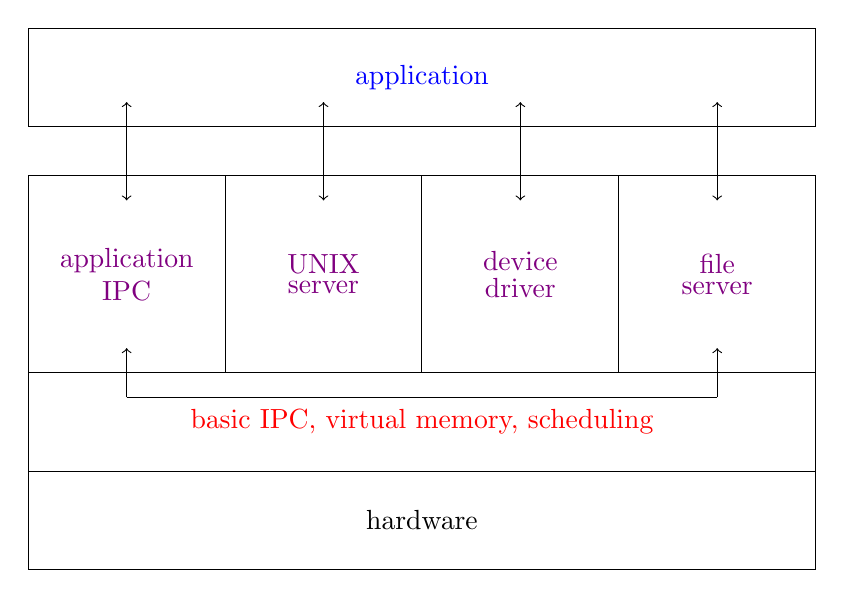
\begin{tikzpicture}[x=2.5cm, y=1.25cm]
                                \node[blue] at (2, -0.5) {application};
                                \node[violet] at (0.5, -2.5) {\shortstack{application\\IPC}};
                                \node[violet] at (1.5, -2.5) {\shortstack{UNIX\\server}};
                                \node[violet] at (2.5, -2.5) {\shortstack{device\\driver}};
                                \node[violet] at (3.5, -2.5) {\shortstack{file\\server}};
                                \node[red] at (2, -4) {basic IPC, virtual memory, scheduling};
                                \node at (2, -5) {hardware};

                                \draw
                                (0.5, -0.75) edge[<->] (0.5, -1.75)
                                (1.5, -0.75) edge[<->] (1.5, -1.75)
                                (2.5, -0.75) edge[<->] (2.5, -1.75)
                                (3.5, -0.75) edge[<->] (3.5, -1.75)
                                (0.5, -3.75) edge[->] (0.5, -3.25)
                                (3.5, -3.75) edge[->] (3.5, -3.25)
                                (0.5, -3.75) -- (3.5, -3.75);

                                \draw (0, 0) -- (4, 0) -- (4, -1) -- (0, -1) -- cycle;
                                \draw (0, -1.5) -- (4, -1.5) -- (4, -3.5) -- (0, -3.5) -- cycle
                                (1, -1.5) -- (1, -3.5)
                                (2, -1.5) -- (2, -3.5)
                                (3, -1.5) -- (3, -3.5);
                                \draw (0, -3.5) -- (0, -4.5) -- (4, -4.5) -- (4, -3.5);
                                \draw (0, -4.5) -- (0, -5.5) -- (4, -5.5) -- (4, -4.5);
                            \end{tikzpicture}
                        \end{center}
                        Note that both the \blue{application} and \violet{servers} run in user mode, and the \red{kernel} is in kernel mode.
                        The kernel performs IPC between the servers, which are separated for device I/O, scheduling. file access etc.
                        \begin{center}
                            \begin{minipage}[t]{0.45\textwidth}
                                advantages
                                \begin{itemize}
                                    \itemsep0em
                                    \item less complex kernel
                                    \item clean interfaces for the servers
                                    \item more reliable; one of the servers could crash and then restart, without bringing the entire kernel down
                                \end{itemize}
                            \end{minipage}
                            \hfill
                            \begin{minipage}[t]{0.45\textwidth}
                                disadvantages
                                \begin{itemize}
                                    \itemsep0em
                                    \item performance overhead due to the requirement of message passing and transitioning between user mode and kernel mode (checks must be done to maintain the separation) - less of an issue now due to better hardware (e.g \textit{Android})
                                \end{itemize}
                            \end{minipage}
                        \end{center}
                    \item \textbf{hybrid kernel} \hfill many modern designs use a combination of both
                        \medskip

                        This is a more structured design, however user-level servers can incur a performance penalty.
                \end{itemize}
            \subsubsection*{Linux Kernel}
                The structure of Linux system calls is to put arguments into registers Or on the stack, and then issue a trap to switch the CPU from user to kernel mode.
                \medskip

                While C is the dominant language for the Linux kernel, the interrupt handlers are written in assembly, as they are low level pieces of code, and require fast performance (hence a low instruction count).
                Interrupt handlers are the primary means to interact with devices, it initiates dispatching which stops proxies, saves the state, starts the driver and returns.
                \medskip

                Typically, we can split the Linux kernel into three parts;
                \begin{itemize}
                    \itemsep0em
                    \item \textbf{I/O}
                        \medskip

                        One of the design philosophies under UNIX style operating system is to treat everything as a file, and use this file abstraction to expose different resources.
                        Therefore, a lot of I/O resources can be hidden under this virtual file system.
                    \item \textbf{memory management}
                        \medskip

                        Includes virtual memory with paging (and the abstractions associated with that).
                    \item \textbf{process management}
                        \medskip

                        Includes process and thread abstraction, as well as synchronisation and scheduling between them.
                \end{itemize}
                In addition to this, Linux supports dynamically loaded modules into the kernel.
                This support was important as it allowed for the hardware configuration to change (new devices drivers could be loaded into the kernel, without recompiling).
            \subsubsection*{Windows Kernel}
                The NTOS kernel layer implements Windows system call interface.
                This is an example of a hybrid kernel, as programs build on dynamic code libraries (DLLs) - which also make the kernel modular, however the executive servers in the kernel adopted the server model of the microkernel, but still runs in kernel space for the performance benefits.
                At the lower levels, there still exists a microkernel.
                In addition, there is also a hardware abstraction layer (HAL), as this was designed for portability.
                \medskip

                It's also important to note that there are environment subsystems running in user mode allowing for different APIs to be exposed, including Win32, POSIX, and OS/2.
                While the Windows kernel was designed with a lot of flexibility, due to its nature as proprietary software, it only really focused support (until recently) on Win32 (and also Intel in terms of the HAL).
        \subsection*{9th October 2020}
            \subsubsection*{Tutorial Questions}
                \begin{enumerate}[1.]
                    \itemsep0em
                    \item Why is the separation into a user mode and a kernel mode considered good OS design?
                        \medskip

                        Reduce the amount of code running in kernel mode, since a bug in user mode code should not bring down the entire system.
                    \item Which of the following instructions should only be allowed in kernel mode, and why?
                        \begin{enumerate}[(a)]
                            \itemsep0em
                            \item disable all interrupts \hfill only kernel mode
                                \subitem if a user program were to disable interrupts, it would prevent the OS from scheduling processes
                            \item read the time of day clock \hfill not privileged
                            \item change any memory \hfill only kernel mode
                                \subitem typically programs can only access its own memory, such that it cannot accidentally or maliciously interfere with other memory
                            \item set the time of day \hfill typically kernel
                                \subitem most programs assume monotonicity of the clock, and changing to an earlier time can cause bugs
                        \end{enumerate}
                    \item Give an example in which the execution of a user process switches from user mode to kernel mode, and then back to user mode.
                        \medskip

                        Reading a file.
                        Essentially anything that requires a system call, as it requires a switch from user mode to kernel mode, and then back.
                    \item A portable operating system is one that can be ported from one system architecture to another with little modification - explain why it is infeasible to build an OS that is portable without any modification.
                        \medskip

                        At some point in the kernel, it will need to know about the ISA (instruction set architecture) of the CPU (hardware), and what instructions it can support.
                        Some parts of the OS require assembly, and therefore requires modification.
                        The hardware abstraction layer in the Windows kernel makes this easier.
                \end{enumerate}
            \subsubsection*{Processes}
                One of the oldest abstractions in computing.
                This is an instance of a program being executed - this is useful as we can then execute multiple programs "simultaneously" on one processor, especially if not all resources are needed at the same time.
                This provides isolation between programs (own address space), and therefore doesn't interfere with other unrelated processes - if it needs to, then the IPC provided can be used.
                It also makes programming easier, as a programmer can assume it is the only process running.
            \subsubsection*{Concurrency}
                It's important to note that there exists both pseudo-concurrency (on one CPU core), as well as real concurrency (across multiple CPU cores).
                The latter will still use the former per core, as the number of processes is much higher than the number of physical cores.
                In the case of multiple cores, we have to deal with conflicting accesses, whereas in the case with a single core, there is only one process really running at a time.
                \medskip

                One method of creating the illusion of concurrency is time slicing.
                The OS switches the process currently running on the CPU with another runnable process, saving the original process' execution state, and then restoring it after it is switched back.
                Note that a runnable process isn't waiting for input, as we want to minimise the amount of time the CPU is idle.
                We also must ensure that the switching is fair - for example, if process ~A~ has a long execution time, compared to an interactive process ~B~, letting ~A~ run for a long period would cause the interactive process to become unresponsive - therefore the time slice tends to be quite short (how often it lets a process run before switching).
                \begin{enumerate}[1.]
                    \itemsep0em
                    \item If on average a process computes $20\%$ of the time, then with 5 processes, we should have $100\%$ CPU utilisation, right?
                        \medskip

                        Only in the ideal case, when they never wait for I/O at the same time.
                        A better estimate is to look at the probability (assuming independence), with $n$ being the number of processes, and $p$ being the fraction of time a process is waiting for I/O.
                        The probability that all are waiting for I/O would be $p^n$, and therefore the CPU utilisation would be $1 - p^n$.
                    \item How many processes nee to be running to only waste $10\%$ of CPU if they spend $80\%$ waiting for I/O?
                        \begin{center}
                            $1 - 0.8^n = 0.9 \Rightarrow 0.8^n = 0.1 \Rightarrow n = \log_{0.8}(0.1) \approx 10$ concurrent processes
                        \end{center}
                \end{enumerate}
            \subsubsection*{Context Switches}
                A context switch is when the processor switches execution from process ~A~ to process ~B~.
                This is done as part of a scheduling decision.
                With timer interrupts, the currently executing program passes control back to the kernel, which can then make a scheduling decision, changing what is currently running, possibly a different program and performing a context switch.
                This causes the order of execution between processes to become non-deterministic, as these events cannot be pre-determined.
                \medskip

                This needs to be transparent to the process, therefore the state needs to be restored exactly, including anything currently in registers (this is saved by the hardware to the stack, before the hardware invokes the interrupt handler).
                This data is stored in a process descriptor, or a process control block (PCB), kept in the process table.
                The process has its own virtual machine;
                \begin{itemize}
                    \itemsep0em
                    \item own virtual CPU
                    \item own address space (stack, heap, text, data, etc.)
                    \item resources it has access to (open file descriptors, etc.)
                \end{itemize}
                The information in registers (such as the program counter, page table register, stack pointer, etc), the process management information (process ID, parents, etc.), as well as file management information also needs to be stored (root directory, working directory, file descriptors, etc.).
                \medskip

                It's also important to avoid unnecessary context switches as they are expensive, not just from the direct cost of managing state, but also the indirect cost to caching (as the old cache contents are no longer relevant).
                Therefore it has to balance fairness, and the frequency of context switches.
            \subsubsection*{Process Lifecycle}
                Processes are created at the startup of a system, by the request of a user, or through a specific system call by a running process.
                These processes can be foreground processes, that the user interacts with, or background processes that provide services (such as printing or mail) or APIs that can be used by other processes (daemons).
                \medskip

                A process can terminate under these conditions;
                \begin{itemize}
                    \itemsep0em
                    \item normal completion, where the process completes execution
                    \item through a system call (~exit()~ in UNIX or ~ExitProcess()~ in Windows)
                    \item abnormal exit, where the process has run into an error or unhandled exception - this is the importance of user and kernel space separation
                    \item aborted, due to another process overruling its execution (such as killing from terminal)
                    \item never - some processes such as daemons should run infinitely and never terminate (unless an error occurs)
                \end{itemize}
                UNIX allows for a process hierarchy (tree), by running ~init~ (typically), and all processes then form a tree.
                On the other hand, Windows has no notion of hierarchy, and rather the parent of a child process is given a token (a handle) to control it.
                This handle can be passed to another process.
        \subsection*{10th October 2019}
            \subsubsection*{UNIX Processes (fork)}
                In UNIX ~int fork(void)~ creates a new child process, which is an exact copy of the parent process, inheriting all resources, and executed concurrently - however, different virtual address space.
                ~fork~ will return twice, however in the parent process it will return the child's process ID, but in the child it will return 0, thus the child knows it's the child.
                Additionally, if there is an error (such as exceeding the global process limit, or running out of memory when copying the parent), -1 will be returned to the parent.
                \begin{lstlisting}
                    #include <unistd.h>
                    #include <stdio.h>

                    int main() {
                      if (fork() != 0) {
                        printf("parent\n");
                      } else {
                        printf("child\n");
                      }
                      printf("common\n");
                    }
                \end{lstlisting}
                The parent and child processes start off with the same memory, but as they start writing to their own memory, they will diverge.
                In the tutorial question below, we'd end up with the following process tree (imagine the spaces in the strings are actually new lines);
                \begin{center}
                    \begin{minipage}[h]{0.485\textwidth}
                        \begin{lstlisting}
                            #include <unistd.h>
                            #include <stdio.h>

                            int main() {
                              if (fork() != 0)
                                printf("X\n");
                              if (fork() != 0)
                                printf("Y\n");
                              printf("Z\n");
                            }
                        \end{lstlisting}
                    \end{minipage}
                    \hfill
                    \begin{minipage}[h]{0.485\textwidth}
                        \begin{center}
                            \begin{tikzpicture}
                                \node[label=right:{\violet{~"X Y Z"~}}] (1) at (0, 0) {1};
                                \node[label=left:{\violet{~"Y Z"~}}] (2) at (-1, -1) {2};
                                \node[label=right:{\violet{~"Z"~}}] (3) at (1, -1) {3};
                                \node[label=right:{\violet{~"Z"~}}] (4) at (-1, -2) {4};

                                \draw
                                (1) edge[->] (2)
                                (1) edge[->] (3)
                                (2) edge[->] (4);
                            \end{tikzpicture}
                        \end{center}
                    \end{minipage}
                \end{center}
                However, note that because this creates new processes that run in parallel, the actual order of execution would be non-deterministic, and therefore the outputs can change the order in which they are printed.
            \subsubsection*{UNIX Processes (execve)}
                While ~fork~ creates a copy of the parent process, we often want the child process to do something different; ~int execve(const char *path, char *const argv[], char *const envp[])~.
                \begin{itemize}
                    \itemsep0em
                    \item ~path~ \hfill full path name of the program to run
                    \item ~argv~ \hfill arguments passed to main
                    \item ~envp~ \hfill environment variables such as ~\$PATH~ and ~\$HOME~
                \end{itemize}
                Running this changes the process image, and runs the new process.
                To start a new process, you could fork the current process, and if it is the child, then run ~execve~ to change the image.
                This has many useful wrappers, and ~man execve~ can be used as a reference.
            \subsubsection*{UNIX Processes (waitpid)}
                The example below is an application, a simple command interpreter, for the two functions previously discussed, as well as a use of ~int waitpid(int pid, int* stat, int options)~;
                \begin{lstlisting}
                    while (1) {
                      read_command(command, parameters);
                      if (fork() != 0) {
                        // parent code here
                        waitpid(-1, &status, 0);
                      } else {
                        // child code
                        execve(command, parameters, 0);
                      }
                    }
                \end{lstlisting}
                This suspends the execution of the calling process until the process with PID ~pid~ terminates, or a signal is received.
                If ~pid~ is set to the following values, it can wait for more than one child;
                \begin{itemize}
                    \itemsep0em
                    \item ~-1~ \hfill wait for any child
                    \item ~0~ \hfill any child in the same process group as the caller
                    \item ~-gid~ wait for any child with the process group ~gid~
                \end{itemize}
                This will return the ~pid~ of the terminated process, -1 if it is an error, or 0 if the call is not blocking and no children are terminated.
            \subsubsection*{UNIX Processes (Termination)}
                A process can terminate from itself by executing ~void exit(int status)~, which is also called implicitly once the program completes execution, and obviously does not return in the calling process (instead returns an exit status to the parent process).
                It can also be terminated by another process via ~void kill(int pid, int sig)~, which sends the signal ~sig~ to the process associated with ~pid~.
            \subsubsection*{Design Philosophy}
                The UNIX design philosophy is to be simplistic.
                Having both ~fork~ and ~execve~ allows us to use the small building blocks, which have limited behaviour, to perform more complex tasks.
                This contrasts with Windows' ~CreateProcess()~ which combines both of them, however, it's much more complex and takes 10 parameters.
            \subsubsection*{Process Communication}
                \begin{itemize}
                    \itemsep0em
                    \item \textbf{signals (UNIX)}
                        \medskip

                        Signals are an Inter-Process Communication mechanism, and they work similar to the delivery of hardware interrupts.
                        If a process runs on behalf of root, the superuser, it has the permission to send signals to any process.
                        The kernel can also send signals to any process.
                        Some of the cases for signals being generated are as follows;
                        \begin{center}
                            \begin{tabular}{ll}
                                signal & meaning \\
                                \hline
                                ~SIGINT~ & interrupt from keyboard \\
                                ~SIGABRT~ & abort signal from ~abort~ \\
                                ~SIGFPE~ & floating point exception \\
                                ~SIGSEGV~ & invalid memory reference \\
                                ~SIGPIPE~ & broken pipe: writing to a pipe with no readers \\
                                ~SIGALRM~ & timer signal from ~alarm~ \\
                                ~SIGTERM~ & termination signal
                            \end{tabular}
                        \end{center}
                        The default action for most signals is to terminate the process, however the receiving process may choose to do the following (~SIGKILL~ and ~SIGSTOP~ cannot be ignored / handled);
                        \begin{itemize}
                            \itemsep0em
                            \item ignore it
                            \item handle it manually with a signal handler;
                                \begin{lstlisting}
                                    signal(SIGINT, my_handler);

                                    void my_handler(int sig) {
                                        printf("ignoring SIGINT");
                                    }
                                \end{lstlisting}
                        \end{itemize}
                    \item \textbf{pipes}
                        \medskip

                        This can be considered as a one-way communication channel between two processes.
                        This essentially opens a byte stream from process ~A~ to process ~B~, allowing ~A~ to send data to process ~B~.
                        This is commonly used in the command line, for example ~cat file.txt | grep foobar~ (the output of ~cat~ is now the input for ~grep~).
                        There are two types; unnamed (default) and named (can be referred to).
                        \medskip

                        This is opened with the ~int pipe(int fd[2])~ system call, which returns two file descriptors, the read end being in ~fd[0]~, and the write end being in ~fd[1]~.
                        If the receiver is reading from an empty pipe, it blocks until data is written, and if the sender is writing to a full pipe, it blocks until data is read.
                        The parent typically makes the system call, and then forks the process, passing the file descriptors to the child.
                        The sender should close the read end, and the receiver should close the write end.
                        \medskip

                        A persistent pipe can outlive the process that created it - it is stored on the file system, and has different semantics since it is flushed when read from.
                        \begin{enumerate}[1.]
                            \itemsep0em
                            \item
                                When two processes communicate through a pipe, the kernel allocated a buffer (say 64KB).
                                What happens when the process at the write-end of the pipe attempts to send additional bytes on a full pipe?
                                \medskip

                                It cannot write to the buffer, therefore it will block (and the scheduler will choose another process to run) until the pipe is read from (and therefore freed up space in the buffer).
                            \item What happens when the process at the write-end of the pipe attempts to send additional bytes but the other process already closed the file descriptor associated with the pipe?
                                \medskip

                                The writing process will have an error returned to it.
                            \item
                                The process at the write-end of the pipe wants to transmit a linked list data structure (with one integer field and a "next" pointer) over a pipe?
                                How can it do this?
                                \medskip

                                The data must be serialised (as if it were going through a network).
                                Since all processes have their own address spaces, the pointer would be meaningless.
                        \end{enumerate}
                    \item \textbf{shared memory}
                    \item \textbf{semaphores}
                \end{itemize}
            \subsubsection*{Threads}
                Threads are also an abstraction for execution, but unlike processes, they are execution streams that share the same address space.
                When multithreading is used, each process can contain one or more threads.
                A thread lives within a process.
                \begin{center}
                    \begin{minipage}[t]{0.485\textwidth}
                        per process
                        \begin{itemize}
                            \itemsep0em
                            \item address space
                            \item global variables
                            \item open files
                            \item child processes
                            \item signals
                        \end{itemize}
                    \end{minipage}
                    \hfill
                    \begin{minipage}[t]{0.485\textwidth}
                        per thread
                        \begin{itemize}
                            \itemsep0em
                            \item program counter (PC)
                            \item registers
                            \item stack
                        \end{itemize}
                    \end{minipage}
                \end{center}
                Threads allow for programs to execute in parallel, but more importantly they can block independently, therefore blocking in one part of the program (waiting for I/O, etc) does not affect the rest of it.
                This is useful, over having many processes, as processes have too much overhead, it is difficult to communicate between address spaces, and anything that blocks may switch out the entire application.
                \medskip

                However, there can be issues with multiple threads.
                Since we are working with the same address space, we need to handle synchronisation, and prevent threads from interfering with each other accidentally (such as stack corruption).
                \medskip

                Typically, when a ~fork~ is performed from a thread, only a single thread is created - however this can lead to issues if the parent is holding locks, the thread now also holds them.
                Generally, we want to avoid calling ~fork~ in a thread.
                While signalling and threading are compatible, there are many corner cases which can complicate the implementation.
            \subsubsection*{PThreads}
                Posix Threads are defined by IEEE standard 1003.1c, and is implemented by most UNIX systems.
                \begin{lstlisting}
                    #include <pthread.h>
                    #include <sys/types.h>

                    pthread_t // type representing a thread
                    pthread_attr_t // type representing the attributes of a thread
                \end{lstlisting}

                Creating a thread is done with ~int pthread\_create(pthread\_t *thread, const pthread\_attr\_t *attr, void *(*start\_routine)(void*), void *arg)~.
                It stores the newly created thread in ~*thread~, and returns 0 if it was created successfully, or an error code otherwise (possibly due to lack of memory, due to the need for a stack).
                A function pointer is also required, as the thread will run the specified function with the arguments provided.
                The arguments are as follows;
                \begin{itemize}
                    \itemsep0em
                    \item ~attr~ \hfill specifies attributes (~NULL~ for default)
                        \subitem such as minimum stack size, behaviour on process termination, etc.
                    \item ~start\_routine~ \hfill C function the thread will start executing
                    \item ~arg~ \hfill argument to be passed into ~start\_routine~ (can be ~NULL~ if none)
                        \subitem if we want to pass in more arguments, pass in a struct, since it is in the same address space
                \end{itemize}
                A thread can be terminated with ~pthread\_exit(void *value\_ptr)~, which terminates the thread, and makes the ~value\_ptr~ available to any successful join (this is fine as threads reside in the same address space).
                \medskip

                It's also important to note that a thread is automatically allocated for the main entry point (starting ~main()~).
                If the main thread terminates without calling ~pthread\_exit()~, the entire process is terminated, however if it does call it, the remaining threads continue until termination (or ~exit()~ is called).
                \medskip

                Yielding a thread with ~int pthread\_yield(void)~ would be done for the same reasons as the system call ~nice()~ is done for processes (lowering priority in the scheduler).
                It releases the CPU to let another thread run, and will always return 0 (success) on Linux.
                \medskip

                In order to join threads, ~int pthread\_join(pthread\_t thread, void **value\_ptr)~ can be used.
                This blocks the caller until ~thread~ terminates, and the value can be accessed.
                \medskip

                All of the content mentioned before assumes a kernel-level thread, such that all of the scheduling is managed by the kernel.
                However, a process can manage its own user-level threads.
                Threads in user-level tend to be more lightweight, as there is very low overhead of context switching, and synchronisation is fast.
                However, because it not visible to the kernel, it may preempt all the threads controlled by a process, instead of just a single one - if one of the threads perform a blocking system call, none of the other threads can run.
            \subsubsection*{Tutorial Question}
                In this question, you are to compare reading a file using a single-threaded file server and a multithreaded server, running on a single-CPU machine.
                It takes 15ms to get a request for work, dispatch it, and do the rest of the necessary processing assuming that the data needed are in the block cache.
                A disk operation is needed $\frac{1}{3}$ of the time, requiring an additional 75ms, during which time the thread sleeps.
                Assume that thread switching time is negligible.
                How many requests per second can the server handle if it is;
                \begin{itemize}
                    \itemsep0em
                    \item single-threaded?
                        \medskip

                        In this case, we should take the weighted average; in a cache hit, it takes the 15ms for the request.
                        However, in a cache miss, it takes the 15ms, as well as the additional I/O operation, which gives a total of 90ms.
                        Taking the weighted average, with the probability given, it takes 40ms.
                        This means that it can perform 25 requests per second.
                    \item multithreaded?
                        \medskip

                        Each request needs 15ms of CPU time, and an average of ($\frac{1}{3} \cdot 75=$)25ms I/O time.
                        Therefore, the probability of a thread being blocked is $\frac{25}{40} = \frac{5}{8}$, as 25ms of the total 40ms is I/O.
                        Assuming that they are independent, the probability of all $n$ threads sleeping is $\frac{5}{8}^n$.
                        \medskip

                        With $100\%$ CPU utilisation, we can do $\frac{1000}{15}$ requests per second, and therefore with the blocking, we will do
                        $$\left(1 - \frac{5}{8}^n\right) \cdot \frac{1000}{15} \text{ requests per second}$$
                \end{itemize}
        \subsection*{17th October 2019}
            This starts with the tutorial question in the last lecture.
            \subsubsection*{Kernel Threads}
                The advantages of kernel threads are that it can easily accommodate blocking calls, such as I/O, allowing for other threads in the process to be scheduled.
                However, this has more scheduling overhead, as we need to transition to and from kernel space.
                This also causes synchronisation to become more expensive, as well as switching before more expensive (still remains cheaper than process switches).
                We are also stuck with what the kernel gives us in terms of scheduling.
                \medskip

                An approach for to take advantage of both types of threads is to use kernel threads and multiplex user-level threads onto some / all of the kernel threads.
                This allows multiple user threads on a single kernel thread.
                \begin{enumerate}[1.]
                    \itemsep0em
                    \item
                        If in a multithreaded web server the only way to read from a file is the normal blocking ~read()~ system call, do you think user-level threads or kernel-level threads are being used?
                        \medskip

                        Kernel-level thread, as it loses the point of being a multithreaded web server if the entire application blocks on a file read.
                \end{enumerate}
            \subsubsection*{Process States}
                The states of a process are as follows;
                \begin{itemize}
                    \itemsep0em
                    \item new \hfill the process is being created
                    \item ready \hfill runnable and waiting for the processor
                    \item running \hfill executing on a processor
                    \item waiting (blocked) \hfill waiting for an event
                    \item terminated \hfill process is being deleted
                \end{itemize}
                \begin{center}
                    \begin{tikzpicture}[x=2cm, y=2cm]
                        \node (nw) at (0, 0) {new};
                        \node (rd) at (2, 0) {ready};
                        \node (rn) at (4, 0) {running};
                        \node (tr) at (6, 0) {terminated};
                        \node (wt) at (4, -1) {waiting};

                        \draw
                        (nw) edge[->, above] node{(1)} (rd)
                        (rd) edge[->, above, bend right=30] node{(2)} (rn)
                        (rn) edge[->, above] node{(3)} (tr)
                        (rn) edge[->, above, bend right=30] node{(4)} (rd)
                        (rn) edge[->, right] node{(5)} (wt)
                        (wt) edge[->, below, bend left=30] node{(6)} (rd);
                    \end{tikzpicture}
                \end{center}
                \begin{enumerate}[(1)]
                    \itemsep0em
                    \item once the process has been initialised / enabled (PCB created) and exists as an entity
                    \item selected by the scheduler to execute
                    \item exits in some way
                    \item preempted - scheduler decides to stop running a process on a CPU core and returns it to the ready state
                    \item performing some blocking I/O operation
                    \item after the blocking operation completes
                \end{enumerate}
            \subsubsection*{Scheduling}
                The states above are for a single process, and as such, multiple processes can be in the ready state (able to run on a CPU core, but not running).
                The job of the scheduler is to decide which one should run.
                A scheduling algorithm has the following properties;
                \begin{itemize}
                    \itemsep0em
                    \item ensure fairness \hfill all processes are "competing" for CPU time
                    \item avoid starvation \hfill no process should never be assigned to the running state
                    \item enforce policy \hfill may need to respect priorities
                    \item maximise resource utilisation \hfill make sure all CPU cores are busy
                    \item minimise overhead
                    \item system specific;
                        \begin{itemize}
                            \itemsep0em
                            \item batch systems \hfill e.g. a compute cluster
                                \subitem we want to minimise the time between job submission and completion (turnaround time), and maximise throughput (the number of jobs per unit of time)
                            \item interactive systems \hfill desktop system with UI
                                \subitem we want fast response times
                            \item real-time systems
                        \end{itemize}
                \end{itemize}
                We also need to consider the types of scheduling;
                \begin{center}
                    \begin{minipage}[t]{0.485\textwidth}
                        non-preemptive
                        \begin{itemize}
                            \itemsep0em
                            \item cannot stop it until it stops itself
                            \item let a process run until it blocks or voluntarily releases CPU
                        \end{itemize}
                    \end{minipage}
                    \hfill
                    \begin{minipage}[t]{0.485\textwidth}
                        preemptive (most modern operating systems)
                        \begin{itemize}
                            \itemsep0em
                            \item let a process run for a maximum amount of fixed time
                            \item requires a clock interrupt
                        \end{itemize}
                    \end{minipage}
                \end{center}
                We can also classify the nature of processes;
                \begin{center}
                    \begin{minipage}[t]{0.485\textwidth}
                        CPU-bound
                        \begin{itemize}
                            \itemsep0em
                            \item bottlenecked resource is the CPU (most of the time it is doing computation)
                            \item performance limited by how fast it can run computations
                        \end{itemize}
                    \end{minipage}
                    \hfill
                    \begin{minipage}[t]{0.485\textwidth}
                        I/O-bound
                        \begin{itemize}
                            \itemsep0em
                            \item occasionally uses CPU
                            \item most of time is spent waiting for I/O
                            \item for example, a terminal waiting for user to enter command
                        \end{itemize}
                    \end{minipage}
                \end{center}
                Some common scheduling algorithms are as follows;
                \begin{itemize}
                    \itemsep0em
                    \item \textbf{first-come-first-served} (non-preemptive)
                        \medskip

                        The ready state is kept as a queue, and new processes are added to the back of the queue.
                        The head of the queue is the next process to be scheduled, and when a waiting process finishes waiting it is added to the back of the queue.
                        \begin{center}
                            \begin{minipage}[t]{0.45\textwidth}
                                advantages
                                \begin{itemize}
                                    \itemsep0em
                                    \item no indefinite postponement as all processes are eventually scheduled
                                    \item very easy to implement
                                \end{itemize}
                            \end{minipage}
                            \hfill
                            \begin{minipage}[t]{0.45\textwidth}
                                disadvantages
                                \begin{itemize}
                                    \itemsep0em
                                    \item in the case a long job is followed many short jobs, head of line blocking occurs, and the average turnaround time suffers
                                \end{itemize}
                            \end{minipage}
                        \end{center}
                    \item \textbf{round-robin scheduling}
                        \medskip

                        The general structure is similar to first-come-first-served, but we have the addition of preemption.
                        We keep a process running until it blocks (like in FCFS), but we also preempt it, and place it in the back of the ready queue, once it exceeds some time quantum.
                        \begin{center}
                            \begin{minipage}[t]{0.45\textwidth}
                                advantages
                                \begin{itemize}
                                    \itemsep0em
                                    \item fair due to ready jobs getting equal share of CPU
                                    \item good response time for a small number of jobs
                                \end{itemize}
                            \end{minipage}
                            \hfill
                            \begin{minipage}[t]{0.45\textwidth}
                                disadvantages
                                \begin{itemize}
                                    \itemsep0em
                                    \item low turnaround time when run-times are different (a short job would need less time quanta)
                                    \item poor turnaround time when run-times are similar (all finish at the same time)
                                \end{itemize}
                            \end{minipage}
                        \end{center}
                        However, we need to decide on the round robin quantum (time slice).
                        For example, with a quantum of 4ms, and 1ms for context switching, 20\% of the time becomes overhead.
                        For a 1s quantum, only 0.1\% is overhead.
                        Therefore for large quantum, there is less overhead, but a worse response time (as the quantum approaches infinity, we go back to FCFS).
                        The reverse is true for small quantum.
                        The typical values lie between 10ms-200ms, Linux uses 100ms, Windows client uses 20ms, and Windows server uses 180ms.
                    \item \textbf{shortest job first} (non-preemptive)
                        \medskip

                        If we know all the run-times in advance, we can pick the jobs that require the least CPU time first.
                        This method is optimal when all the jobs are given simultaneously,
                    \item \textbf{shortest remaining time}
                        \medskip

                        This is a preemptive version of SJF - when a new process arrives with a shorter execution time than the remaining time for the currently running process, it should be run.
                        This allows new short jobs to get good service.
                        \medskip

                        However, these two methods require knowing the run-times, which isn't always possible.
                \end{itemize}
                Some scheduling algorithms take priority into account (priority scheduling).
                The priority of a job may be defined by the user, or based on some metrics determined by the OS.
                They can also be static (and remain constant) or dynamic (changes during execution).
                The goal is to run jobs based on their priority.
                \medskip

                In general, we want to favour short and I/O bound jobs - this allows for good resource utilisation and short response times (I/O bound jobs are waiting anyways, and therefore don't need much CPU time).
                A general-purpose scheduler can quickly determine the nature of a certain job, and then adapt to those changes.
            \subsubsection*{Multilevel Feedback Queues (MLFQ)}
                A form of priority scheduling is a multilevel feedback queue, which is implemented by many operating systems.
                This has a queue for each priority level, and runs a job from the highest non-empty priority queue, usually using round-robin.
                However, this has the issue that if high priority jobs keep being added, then something of a lower priority might never be run, leading to starvation.
                A way around this is to have a feedback mechanism in place, where the job priority is recomputed periodically based on how much CPU they have used recently.
                This is an exponentially-weighted moving average.
                Additionally, a job's priority it should increase as it waits.
                \medskip

                However, this has a few drawbacks;
                \begin{itemize}
                    \itemsep0em
                    \item priorities make no guarantees - assume a system of 16 queues, and a job is given a priority of 15, this can mean nothing if there are many jobs of priority 16
                    \item priority assignment requires a warm-up period, when the operating system needs to work out what the job does
                    \item cheating is a concern - a program may issue I/O requests to boost priority
                    \item cannot donate priority
                \end{itemize}
            \subsubsection*{Lottery Scheduling}
                By \textit{Waldspurger and Weihl}.
                Jobs receive lottery tickets for the resources they need (such as CPU time).
                At each scheduling decision, one ticket is chosen at random, and the job holding that ticket wins.
                Priorities in this scheme are done by biasing the number of tickets - in a system with 100 tickets for CPU time, and giving a job 20 tickets means that it will have 20\% of the CPU time in the long run.
                This also has additional nice properties;
                \begin{itemize}
                    \itemsep0em
                    \item no starvation (as every job will almost certainly be done at some point)
                    \item highly responsive, as it will have the number of tickets needed to get a certain percentage chance of getting the resource at the \textbf{next} decision
                    \item supports priority donation, as a process can give tickets to another
                    \item adding jobs / removing jobs affects other jobs proportionally
                \end{itemize}
                However, the main obvious drawback is the unpredictable response time, and if an interactive process is unlucky, it can be unresponsive.
        \subsection*{23rd October 2019}
            \subsubsection*{Tutorial Questions}
                State which of the following are true and which are false, justifying answers.
                \begin{enumerate}[1.]
                    \itemsep0em
                    \item Interactive systems generally use non-preemptive processor scheduling.
                        \medskip

                        False.
                        They use preemptive scheduling to guarantee a fast response to new requests.
                        Service trivial, I/O-bound, interactive requests quickly.
                    \item Turnaround times are more predictable in preemptive than in non-preemptive systems.
                        \medskip

                        False.
                        In non-preemptive systems, a process will run to completion or until it blocks once it gets a processor.
                    \item One weakness of priority scheduling is that, while a system may faithfully honour the priorities, the priorities themselves may not be meaningful.
                        \medskip

                        True.
                        The (actual) priority of a job, and how meaningful it is, often depends on what other jobs are running.
                \end{enumerate}
            \subsubsection*{Synchronisation}
                One example of synchronisation we've already seen is the joining of two ~pthreads~.
                Note that we can often use processes and threads interchangeably, as the concepts are relevant to both.
                A lot of the system calls that the kernel exposes for synchronisation are exposed through programming languages, as the language must have the ability to control threads.
            \subsubsection*{Mutual Exclusion}
                This goes through a standard example of race conditions due to shared data;
                \begin{lstlisting}
                    void extract(int acc, int sum) {
                      int b = accs[acc];
                      accs[acc] = b - sum;
                    }
                \end{lstlisting}
                The code above is a critical section (processes access a shared resource), and we need mutual exclusion (such that ensures that if a process is in a critical section, no other process can execute it, hence processes must request permission to enter).
                Therefore, some synchronisation mechanism is required at the entry and exit of this section.
                The requirements for mutual exclusion are as follows;
                \begin{itemize}
                    \itemsep0em
                    \item no two processes may be simultaneously inside a critical section
                    \item no processes running outside the critical section may prevent other processes from entering the critical section (any process requesting permission to enter should be allowed to when there is no process inside that section)
                    \item no process should be delayed from entering the critical section forever
                    \item cannot assume about the progress of processes (while it may be easy to assume that two threads are making the same progress, it is really up to the scheduler)
                \end{itemize}
                \begin{center}
                    \begin{tikzpicture}
                        \node (a) at (0, 0) {process ~A~};
                        \node (b) at (0, -2) {process ~B~};
                        \node (t1) at (3, -3) {$T_1$};
                        \node (t2) at (4, -3) {$T_2$};
                        \node (t3) at (7, -3) {$T_3$};
                        \node (t4) at (9, -3) {$T_4$};

                        \draw
                        (a) -- (3, 0)
                        (7, 0) -- (10, 0)
                        (b) -- (4, -2)
                        (9, -2) -- (10, -2)
                        (3, 0.25) -- (7, 0.25) -- (7, -0.25) -- (3, -0.25) -- cycle
                        (7, -1.75) -- (9, -1.75) -- (9, -2.25) -- (7, -2.25) -- cycle;

                        \draw[dotted]
                        (4, -2) -- (7, -2);

                        \draw[dashed]
                        (3, 0) -- (t1)
                        (4, -0.25) -- (t2)
                        (7, 0) -- (t3)
                        (9, 0) -- (t4);
                    \end{tikzpicture}
                \end{center}
                \begin{enumerate}[$T_1$:]
                    \itemsep0em
                    \item ~A~ enters the critical region
                    \item ~B~ attempts to enter the critical region, ~B~ is blocked
                    \item ~A~ leaves the critical region, ~B~ is unblocked, and enters the critical region
                    \item ~B~ leaves the critical region
                \end{enumerate}
                Some methods of preventing this are as follows;
                \begin{itemize}
                    \itemsep0em
                    \item \textbf{disabling interrupts}
                        \medskip

                        A very simple way of doing this is to disable interrupts;
                        therefore we can have ~CLI()~ before line 2, and ~STI()~ after line 3.
                        As no timer interrupts can occur, the processor cannot context switch to another thread.
                        This has some major issues;
                        \begin{itemize}
                            \itemsep0em
                            \item only works on single-processor systems, as we have true parallelism (such that multiple processes can truly run at the same time - no context switching needed) with multiple processors
                            \item slows down the system, as nothing else can run during that time
                            \item because there is no way for the kernel to take back control, a bug in this critical section cannot be recovered from - this mechanism is typically only used by kernel code
                        \end{itemize}
                    \item \textbf{strict alternation} \hfill software solution
                        \medskip

                        The idea here is to maintain a global ~turn~ variable.
                        While the thread is not on its turn, it simply "busy waits" for the variable to change to its turn.
                        Once it is, it can then assume that any other thread attempting to access the critical section is now waiting in the loop.
                        After it has finished execution, it can change the turn.
                        \begin{center}
                            \begin{minipage}[t]{0.45\textwidth}
                                thread 0
                                \begin{lstlisting}
                                    while (true) {
                                      while (turn != 0)
                                        /* busy wait */;
                                      critical();
                                      turn = 1;
                                      noncritical0();
                                    }
                                \end{lstlisting}
                            \end{minipage}
                            \hfill
                            \begin{minipage}[t]{0.45\textwidth}
                                thread 1
                                \begin{lstlisting}
                                    while (true) {
                                      while (turn != 1)
                                        /* busy wait */;
                                      critical();
                                      turn = 0;
                                      noncritical1();
                                    }
                                \end{lstlisting}
                            \end{minipage}
                        \end{center}
                        This also has issues;
                        \begin{itemize}
                            \itemsep0em
                            \item by doing this we've assumed a form of alternation, that it switches between the threads (switches from thread 0 to thread 1, and vice versa); this means that if thread 0 wishes to enter the critical region again, after finishing a short non-critical region, it must wait for thread 1 to enter the critical region and set ~turn~
                                \subitem thread 1 can take a long time in its non-critical region, causing non-critical code to prevent entry to critical code
                            \item we are also performing a busy wait - this wastes CPU time as we are continuously checking a global variable, therefore we need kernel support to prevent this
                        \end{itemize}
                    \item \textbf{Peterson's solution} \hfill software solution
                        \begin{lstlisting}
                            int turn = 0;
                            int interested[2] = { 0, 0 };

                            void enter_critical(int thread) {
                              int other = 1 - thread; // thread is 0 or 1
                              interested[thread] = 1;
                              turn = other;
                              while (turn == other && interested[other])
                                /* busy wait */;
                            }

                            void leave_critical(int thread) {
                              interested[thread] = 0;
                            }
                        \end{lstlisting}
                        While this still uses the global ~turn~, we have an additional ~interested~ variable.
                        Note that when a thread enters, it marks that it is interested.
                        When both thread 0 and thread 1 attempt to enter the section, turn only allows one thread to enter.
                        If thread 0 is in the critical section, then thread 1 must wait for thread 0 to set interested to 0, which can only happen after thread 0 leaves, and vice versa.
                    \item \textbf{lock variables}
                        \medskip

                        We can utilise a TSL (test and set lock) instruction, which is an atomic instruction provided by most CPUs.
                        ~TSL(LOCK)~ atomically sets the memory location ~LOCK~ to 1, and returns the old value.
                        Note that locks that rely on busy waiting are called \textbf{spin locks} - these can still be used if we have a very short wait time, as we don't need to handle the overhead from context switching.
                        Spin locks are still used by the kernel, as it cannot use a blocking abstraction.
                        \medskip

                        It's also important to consider lock granularity (the amount of data a lock is protecting).
                        Note that in the ~extract~ example at the start, attempting to withdraw from different accounts shouldn't interfere with each other, and therefore it shouldn't be a global lock, but rather a lock per account.
                        \medskip

                        Similarly, we should also consider the overhead of using locks, such as the memory space from storing data about them, the time used for initialisation, and the time needed to acquire and release them.
                        With higher lock contention (the number of processes waiting for a lock), we have less parallelism.
                        \begin{center}
                            \begin{minipage}[t]{0.45\textwidth}
                                coarser granularity
                                \begin{itemize}
                                    \itemsep0em
                                    \item less lock overhead (less locks)
                                    \item more lock contention
                                    \item less complex to implement
                                \end{itemize}
                            \end{minipage}
                            \hfill
                            \begin{minipage}[t]{0.45\textwidth}
                                finer granularity
                                \begin{itemize}
                                    \itemsep0em
                                    \item more lock overhead
                                    \item less lock contention
                                    \item more complex to implement
                                \end{itemize}
                            \end{minipage}
                        \end{center}
                        To maximise concurrency, we need to choose a finer lock granularity (understanding the tradeoffs).
                        The goal is to make the critical sections smaller, and release locks as soon as they aren't needed.
                        For example, in the code below, we should release the outer lock ~L\_accs~ after creating the account, as it is only needed for that part.
                        \begin{lstlisting}
                            void addAccount(int acc, int balance) {
                              lock(L_accs);
                              createAccount(acc);
                              lock(L[acc]);
                              accs[acc] = balance;
                              unlock(L[acc]);
                              unlock(L_accs);
                            }
                        \end{lstlisting}
                        Additionally, we should differentiate between locks held for reading and writing.
                        Two threads attempting to \textbf{read} the same data should be allowed to do so, and it reduces parallel unnecessarily if they block each other.
                        ~lock\_RD(L)~ acquires lock ~L~ in read mode, and ~lock\_WR(L)~ acquires it in write mode.
                        In write mode, no other thread can acquire either a read or a write lock, however multiple threads can acquire a lock in read mode.
                \end{itemize}
            \subsubsection*{Priority Inversion}
                Assume we have two processes, ~H~ and ~L~ with high and low priority, respectively.
                Our scheduler should always schedule ~H~ if it is runnable.
                Now, ~H~ is waiting for I/O, is therefore blocked, and ~L~ is scheduled.
                ~L~ acquires lock ~A~ for a critical section.
                I/O arrives for ~H~, and it is unblocked, ~L~ is preempted and ~H~ is scheduled.
                ~H~ then attempts to acquire lock ~A~, but ~L~ is holding that lock.
                \medskip

                If we were to use a busy wait in software, the kernel does not know that ~H~ is blocked, and will continue to schedule it, thus not allowing ~L~ to be scheduled, and the lock is never released.
                This is called priority inversion, as a higher priority process is being blocked from running by a lower priority process.
                \medskip

                Therefore, preemptive scheduling needs to take into account the lock implementation and mutual exclusion.
            \subsubsection*{Race Condition}
                This occurs when multiple threads or processes read and write shared data, and the final results depends on the relative timing of their execution (on the exact process or thread interleaving).
                \medskip

                Consider the following three threads (tutorial question);
                \begin{enumerate}[~T1~:]
                    \itemsep0em
                    \item ~a = 1; b = 2~
                    \item ~b = 1;~
                    \item ~a = 2;~
                \end{enumerate}
                \begin{enumerate}[1.]
                    \itemsep0em
                    \item How many possible interleavings are there? \hfill 12 interleavings
                    \item If all thread interleavings are as likely to occur, what is the probability to have ~a = 1~, and ~b = 1~ after all threads complete execution?
                        \medskip

                        $\frac{1}{12}$, as ~T2~ must occur after ~T1~, and ~T3~ must occur before ~T1~.
                \end{enumerate}
                From this, we can see why multithreaded applications are difficult to debug, as the results can be unpredictable (and only occasionally cause bugs).
            \subsubsection*{Memory Models}
                It's important to remember that modern CPUs can execute instructions out of order in the interest of performance.
                We've assumed the operation of each thread appear in program order (and each operation executes atomically).
                This is not necessarily what the CPU or the compiler assumes, and can lead to unexpected behaviour.
                Therefore, we should not rely on expected behaviour of a memory model, and just avoid data races (such that they are protected and will work regardless of the model).
                We assume strong memory models in this course.
        \subsection*{24th October 2019}
            \subsubsection*{Happens-Before Relationship}
                In order to formalise the execution of events, we think about instructions that are executed as events in a trace.
                We then have a partial ordering denoted by $a \to b$.
                Consider two events, $a, b$, with $a$ occurring before $b$ in the trace;
                \begin{itemize}
                    \itemsep0em
                    \item if $a$ and $b$ are in the same thread, then $a \to b$
                    \item if $a$ is ~unlock(L)~, and $b$ is ~lock(L)~, then $a \to b$ (this can be used to enforce an ordering between threads)
                \end{itemize}
                This has the following properties;
                \begin{itemize}
                    \itemsep0em
                    \item $\forall a.\ a \not\to a$ \hfill irreflexive
                    \item $\forall a, b.\ a \to b \Rightarrow b \not\to a$ \hfill antisymmetric
                    \item $\forall a, b, c.\ a \to b \land b \to c \Rightarrow a \to c$ \hfill transitive
                \end{itemize}
                Therefore, we can formally define a data race between $a$ and $b$ in the trace if and only if;
                \begin{itemize}
                    \itemsep0em
                    \item they access the same memory location
                    \item at least one is a write
                    \item they are unordered according to the relation we just defined
                \end{itemize}
                When the ordering is drawn, we are assuming a particular execution order between threads (in terms of locks) - for example we can assume ~T1~ runs before ~T2~, and therefore the lock in ~T2~ happens after the unlock in ~T1~, but it can also be the other way around; therefore to notice race conditions we may still need to enumerate the executions.
                \begin{lstlisting}
                    int a, int b;
                    void T1 {                                void T2 {
                      a++;                                     lock(L);
                      lock(L);                                 b++;
                      b++;                                     unlock(L);
                      unlock(L);                               a++
                    }                                        }
                \end{lstlisting}
                This is safe if the ~lock(L)~ in ~T2~ is after the ~unlock(L)~ in ~T1~, however if ~T2~ were to lock first, then there is a data race between ~a++~ in both ~T1~ and ~T2~.
            \subsubsection*{Semaphores}
                A semaphore can be thought of as a signalling mechanism between two threads.
                A process will stop, waiting for a specific signal, and a process will continue if it has received a specific signal.
                The semaphore ~s~ can be accessed via these atomic operations;
                \begin{itemize}
                    \itemsep0em
                    \item ~down(s)~ \hfill waiting to receive a signal
                    \item ~up(s)~ \hfill triggering and sending a signal
                    \item ~init(s, i)~ \hfill initialising a semaphore
                \end{itemize}
                Semaphores have two private components; a counter (which is a non-negative integer), and a queue of processes currently waiting for that semaphore.
                \begin{lstlisting}
                    init(s, i): counter(s) = i
                                queue(s) = { }

                       down(s): if counter(s) > 0
                                  counter(s) = counter(s) - 1
                                else
                                  add P to queue(s)
                                  suspend P

                         up(s): if queue(s) not empty:
                                  resume a process in queue(s)
                                else
                                  counter(s) = counter(s) + 1
                \end{lstlisting}
                This can be used to perform the following;
                \begin{itemize}
                    \itemsep0em
                    \item \textbf{mutual exclusion}
                        \medskip

                        We can use a semaphore to implement mutual exclusion - via the use of a binary semaphore (where we initialise it to 1).
                        Therefore a process can acquire the "lock" with ~down(s)~, perform work in the critical section, and then release the "lock" with ~up(s)~.
                    \item \textbf{ordering events}
                        \begin{lstlisting}
                            process A
                              ...
                              (critical section)
                              up(s)
                              ...
                            end
                            process B
                              ...
                              down(s)
                              (critical section)
                              ...
                            end
                        \end{lstlisting}
                        With the semaphore initialised to 0, this forces ~process A~ to execute its critical section before ~process B~ can execute its critical section, forcing an ordering.
                    \item \textbf{multiple producers and multiple consumers}
                        \medskip

                        You can consider the number of processes that are allowed into the critical region as the initial value of the counter.
                        \medskip

                        Consider the scenario where there is a shared data structure, such as a buffer, a set of producers (threads that are writing into the buffer), and a set of consumers (threads reading from the buffer if there are new elements).
                        We then have the following constraints;
                        \begin{itemize}
                            \itemsep0em
                            \item producer
                                \begin{itemize}
                                    \itemsep0em
                                    \item items can only be deposited in the buffer if there is space (block if it is full)
                                    \item items can only be written if mutual exclusion is ensured (we don't want writes to interfere)
                                \end{itemize}
                            \item consumer
                                \begin{itemize}
                                    \itemsep0em
                                    \item items can only be fetched if buffer is non-empty (block if empty)
                                    \item items can only be read if mutual exclusion is ensured (don't want to read incomplete items)
                                \end{itemize}
                            \item buffer \hfill can hold between 0 and $N$ items
                        \end{itemize}
                        \begin{lstlisting}
                            var item, space, mutex: Semaphore
                            init(item, 0) // signalling between producer and consumer
                            init(space, N) // ^
                            init(mutex, 1) // initialised to 1 to ensure mutual exclusion

                            procedure producer()
                              loop
                                (produce item)
                                down(space)
                                down(mutex)
                                (deposit item)
                                up(mutex)
                                up(item)
                              end
                            end

                            procedure consumer()
                              loop
                                down(item)
                                down(mutex)
                                (fetch item)
                                up(mutex)
                                up(space)
                                (consume item)
                              end
                            end
                        \end{lstlisting}
                        Looking at the producer, we can see it performs the following steps;
                        \begin{enumerate}[(1)]
                            \itemsep0em
                            \item it first produces an item
                            \item it attempts to ~down~ the ~space~ semaphore, it blocks if the buffer is full and will resume once a consumer reads
                            \item it then enters the critical region, deposits the item, and exits
                            \item it ~up~s the ~item~ semaphore, signalling that there is an item
                        \end{enumerate}
                        On the other hand, the consumer does the following;
                        \begin{enumerate}[(1)]
                            \itemsep0em
                            \item it attempts to ~down~ the ~item~ semaphore, if it is 0, there are no items to be read, and will block until a producer deposits
                            \item it then enters the mutual exclusion zone, fetches it, exits, and frees space in the buffer, finally consuming the item
                        \end{enumerate}
                \end{itemize}
            \subsubsection*{Monitors and Condition Variables}
                This is a higher level synchronisation primitive.
                The monitor protects shared data, and has a procedure that must be called to enter the monitor from outside.
                There are then internal procedures that can only be called from monitor procedures (the monitor itself is implicitly protected by a lock), and has one or more condition variables.
                Processes can only call entry procedures, and cannot directly access internal data - one process in the monitor at a time.
                \medskip

                Condition variables are associated with high-level conditions, similar to what we used for the final example in semaphores, such as "some space has become available".
                This can be thought of as a signalling mechanism that something has occurred between two threads.
                It has the following operations;
                \begin{itemize}
                    \itemsep0em
                    \item ~wait(c)~ \hfill release monitor lock, and waits for ~c~ to be signalled
                    \item ~signal(c)~ \hfill wakes up a process waiting for ~c~
                    \item ~broadcast(c)~ \hfill wakes up all processes waiting for ~c~
                \end{itemize}
                Unlike semaphores, signals do not accumulate, therefore if ~signal~ is called with no waiting thread, the signal is lost.
                Hence if ~signal~ was called before ~wait~, then the ~wait~ would have to wait until the next ~signal~ is called (can be indefinite if no ~signal~ is called in the future - this causes bugs if a thread "misses" its signal).
                The same model as above can be done with monitors as follows;
                \begin{lstlisting}
                    monitor ProducerConsumer
                      condition not_full, not_empty
                      int count = 0

                      entry procedure insert(item)
                        while (count == N) wait(not_full) // block until signalled if full
                        insert_item(item)
                        count++
                        signal(not_empty) // wakes up a waiting thread

                      entry procedure remove(item)
                        while (count == 0) wait(not_empty)
                        remove_item(item)
                        count--
                        signal(not_full)
                    end monitor
                \end{lstlisting}
                Note the use of ~while~ as the condition, instead of ~if~ as we always need to re-check the condition.
                There is some subtlety on what happens on a signal;
                \begin{itemize}
                    \itemsep0em
                    \item Hoare \hfill a process waiting for a signal is immediately scheduled
                        \begin{itemize}
                            \itemsep0em
                            \item easy to reason about
                            \item inefficient - the signalling process switches out even if it has not finished yet with the monitor
                            \item places extra constraints on scheduler
                        \end{itemize}
                    \item Lampson \hfill sending signal and waking up from a wait is not atomic
                        \begin{itemize}
                            \itemsep0em
                            \item harder to understand, need to take extra care when waking up from ~wait~ (hence re-checking)
                            \item more efficiently, no constraints on scheduler
                            \item more error tolerant, if condition being notified is wrong, simply discarded when rechecked
                        \end{itemize}
                        This is usually used.
                \end{itemize}
                Two threads in the same process can synchronise using a kernel semaphore only if they are implemented by the kernel, because the kernel needs to be able to see the threads and manipulate them.
            \subsubsection*{Deadlocks}
                A set of processes is deadlocked if each process is waiting for an event that only another process can cause.
                This is similar to a data race in the sense that this may not always happen, and execution may be able to proceed as expected.
                Consider the two processes;
                \begin{center}
                    \begin{minipage}[t]{0.485\textwidth}
                        P0:
                        \begin{lstlisting}
                            down(scanner);
                            down(cd_writer);
                            scan_and_record();
                            up(cd_writer);
                            up(scanner);
                        \end{lstlisting}
                    \end{minipage}
                    \hfill
                    \begin{minipage}[t]{0.485\textwidth}
                        P1:
                        \begin{lstlisting}
                            down(cd_writer);
                            down(scanner);
                            scan_and_record();
                            up(scanner);
                            up(cd_writer);
                        \end{lstlisting}
                    \end{minipage}
                \end{center}
                If P0 downs the ~scanner~, and then it context switches to P1, which downs the ~cd\_writer~, they are in deadlock.
                The each want to down the semaphore the other have downed, but neither can progress.
                For resource deadlock, the most common, these 4 conditions must hold;
                \begin{itemize}
                    \itemsep0em
                    \item mutual exclusion \hfill each resource is either available or assigned to one process
                    \item hold and wait \hfill process can request resources while it holds other resources
                    \item no preemption \hfill resources given cannot be forcibly revoked
                    \item circular wait \hfill two or more processes in a circular chain, waiting for a held resource
                \end{itemize}
                Brief tutorial questions;
                \begin{enumerate}[1.]
                    \itemsep0em
                    \item Can the set of processes deadlocked include processes that are not in the circular chain in the corresponding resource allocation graph?
                        \medskip

                        Yes - a process may be waiting on a resource that is held in a circular chain, but not holding a resource (that's needed in the chain)
                    \item
                        Can a single-processor system have no processes ready and no process running?
                        Is this a deadlocked system?
                        \medskip

                        Yes (all processes waiting for I/O) - but this is not a deadlocked system.
                        Typically, we have an idle process created by the kernel that runs when there are no other processes ready (this powers down the core / lowers the core frequency).
                        Therefore we cannot see if we are in a deadlock just by checking that there are no processes running and none are ready.
                \end{enumerate}
            \subsubsection*{Resource Allocation Graph and Dealing with Deadlocks}
                This is a directed graph that models resource allocation, an arc from a resource to a process means that the process owns that resource, and an arc from a process to a resource means that the process is blocked waiting for that resource.
                If a cycle is present, then there is a deadlock.
                Some strategies are as follows;
                \begin{enumerate}[(1)]
                    \itemsep0em
                    \item \textbf{ignore it} \hfill when it is such a rare occurrence, it can be ignored
                    \item \textbf{detection and recovery}
                        \medskip

                        Dynamically build the resource ownership graph and look for cycles.
                        Mark a visited arc, if we encounter a visited arc, then a cycle is present.
                        \medskip

                        Once we've figured out we have a deadlock, we can preempt a process in the cycle - however this can break the program.
                        A method that is less damaging would be to rollback to a previously checkpointed state, redo the computation, ensuring that the same scheduling decisions aren't made.
                        Another strategy is to kill a random process in the cycle, assuming that the process can handle it.
                    \item \textbf{dynamic avoidance} \hfill decide whether it is safe to grant access to resource when requested
                        \medskip

                        Banker's Algorithm, by \textit{Dijkstra}.
                        Essentially, it models resources available similar to how a bank can give customers (threads) a credit limit, and the bank can reserve less than the sum of all the credit limits.
                        Each process can have less than, or equal to, its limit.
                        \medskip

                        A state is considered safe if there are enough resources to satisfy the maximum request from any customer.
                        This creates some sequence of allocations that guarantees that all customers can be satisfied.
                        For example, in the state below (with 2 free resources), it is safe, as we can satisfy ~C~, which frees all 4 resources, allowing us to satisfy ~B~ or ~D~, and so on.
                        \begin{center}
                            \begin{tabular}{lcc}
                                & has & max \\
                                \hline
                                ~A~ & 1 & 6 \\
                                ~B~ & 1 & 5 \\
                                ~C~ & 2 & 4 \\
                                ~D~ & 4 & 7
                            \end{tabular}
                        \end{center}
                    \item \textbf{prevention} \hfill ensure at least one of the four conditions cannot occur
                \end{enumerate}
\end{document}
